\chapter{Appendix 2: Analysis of the network embedding learned from local structural, global structural, and time components}
\label{appendix:k-means_time_struc}

\section{$k$-means}
~\autoref{fig:App5} shows learned sets of embeddings reduced by three dimensionality reduction techniques.~\autoref{fig:App6} and~\autoref{fig:App7} provide visual insights into the optimal $k$ for $k$-means: PCA - $k$ = 4; t-SNE - $k$ = 4; UMAP - $k$ = 5.~\autoref{fig:App8} demonstrates the clustering results on data sets from ~\autoref{fig:App6}. The best clustering according to the set of internal clustering metrics is UMAP-reduced embeddings split into 5 clusters (right plot on~\autoref{fig:App5}).

\begin{figure}[!ht]
	\centering
	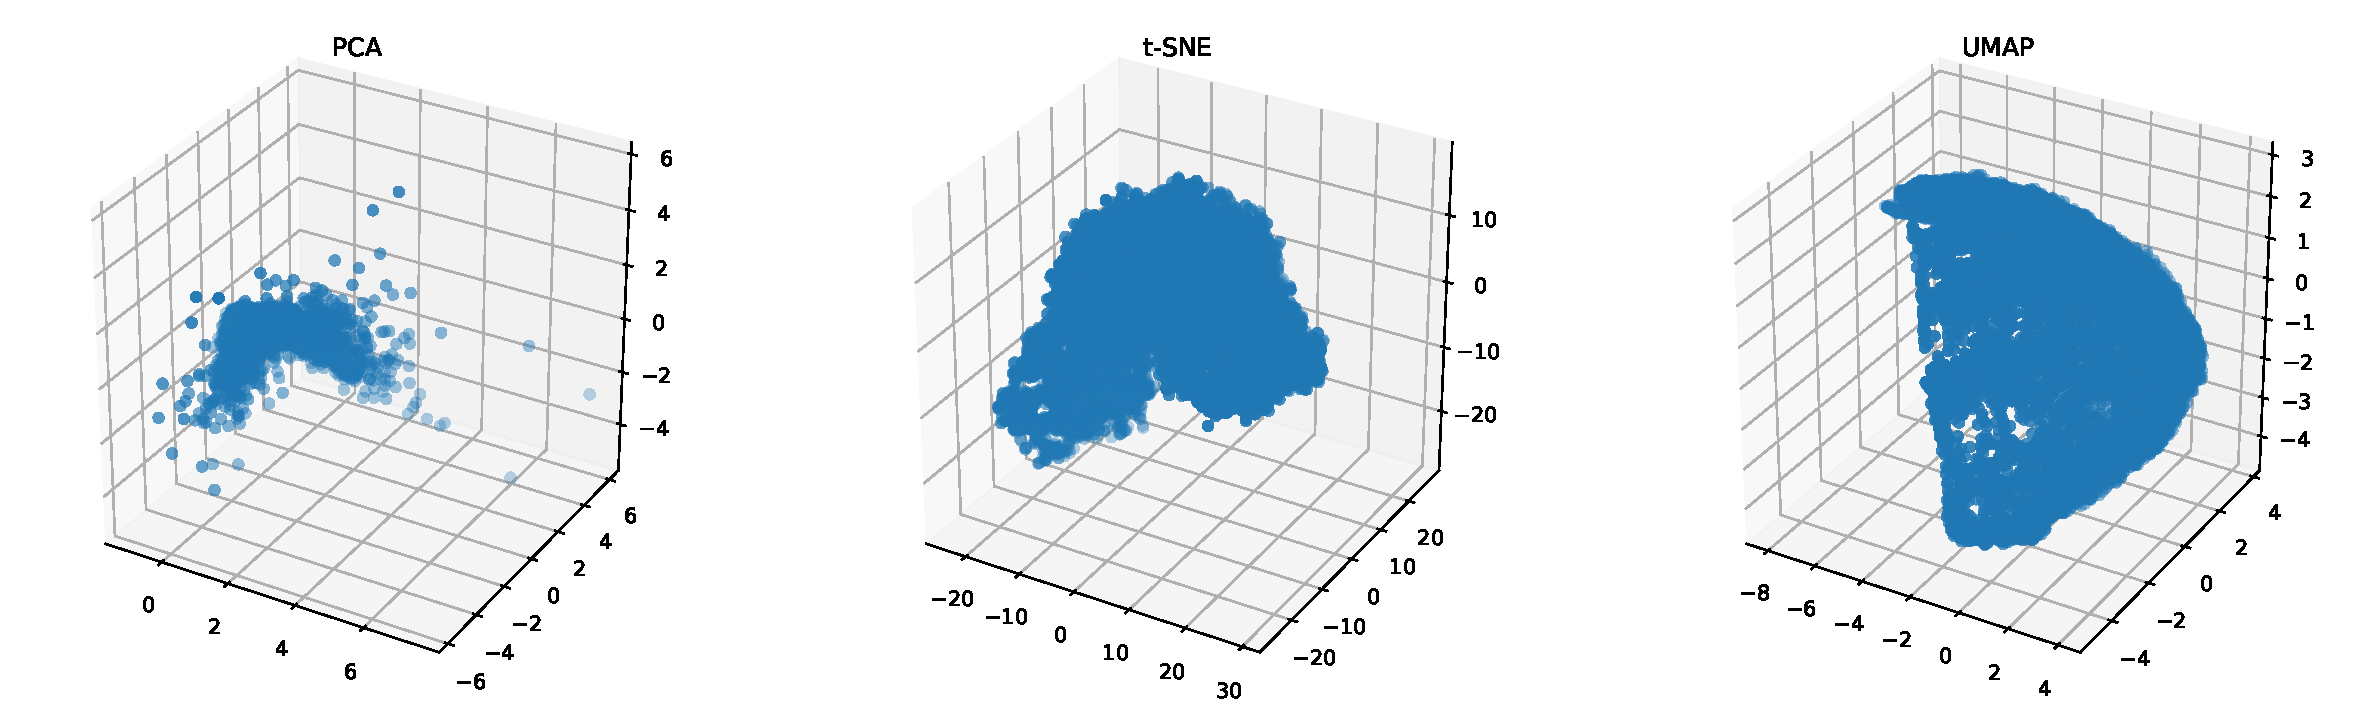
\includegraphics[width=1.0\textwidth]{images/appendix/App5.pdf}\\
	\caption{Embedding set reduced to 3 dimensions by three dimensionality reduction techniques.}
	\label{fig:App5}
\end{figure}
\begin{figure}[!ht]
	\centering
	\includegraphics[width=1.0\textwidth]{images/appendix/App6.pdf}\\
	\caption{Elbow plots for 3-dimensional embedding sets.}
	\label{fig:App6}
\end{figure}
\begin{figure}[!ht]
	\centering
	\includegraphics[width=1.0\textwidth]{images/appendix/App7.pdf}\\
	\caption{Evaluation of $k$-means clustering with respect to the number of clusters $k$.}
	\label{fig:App7}
\end{figure}
\begin{figure}[!ht]
	\centering
	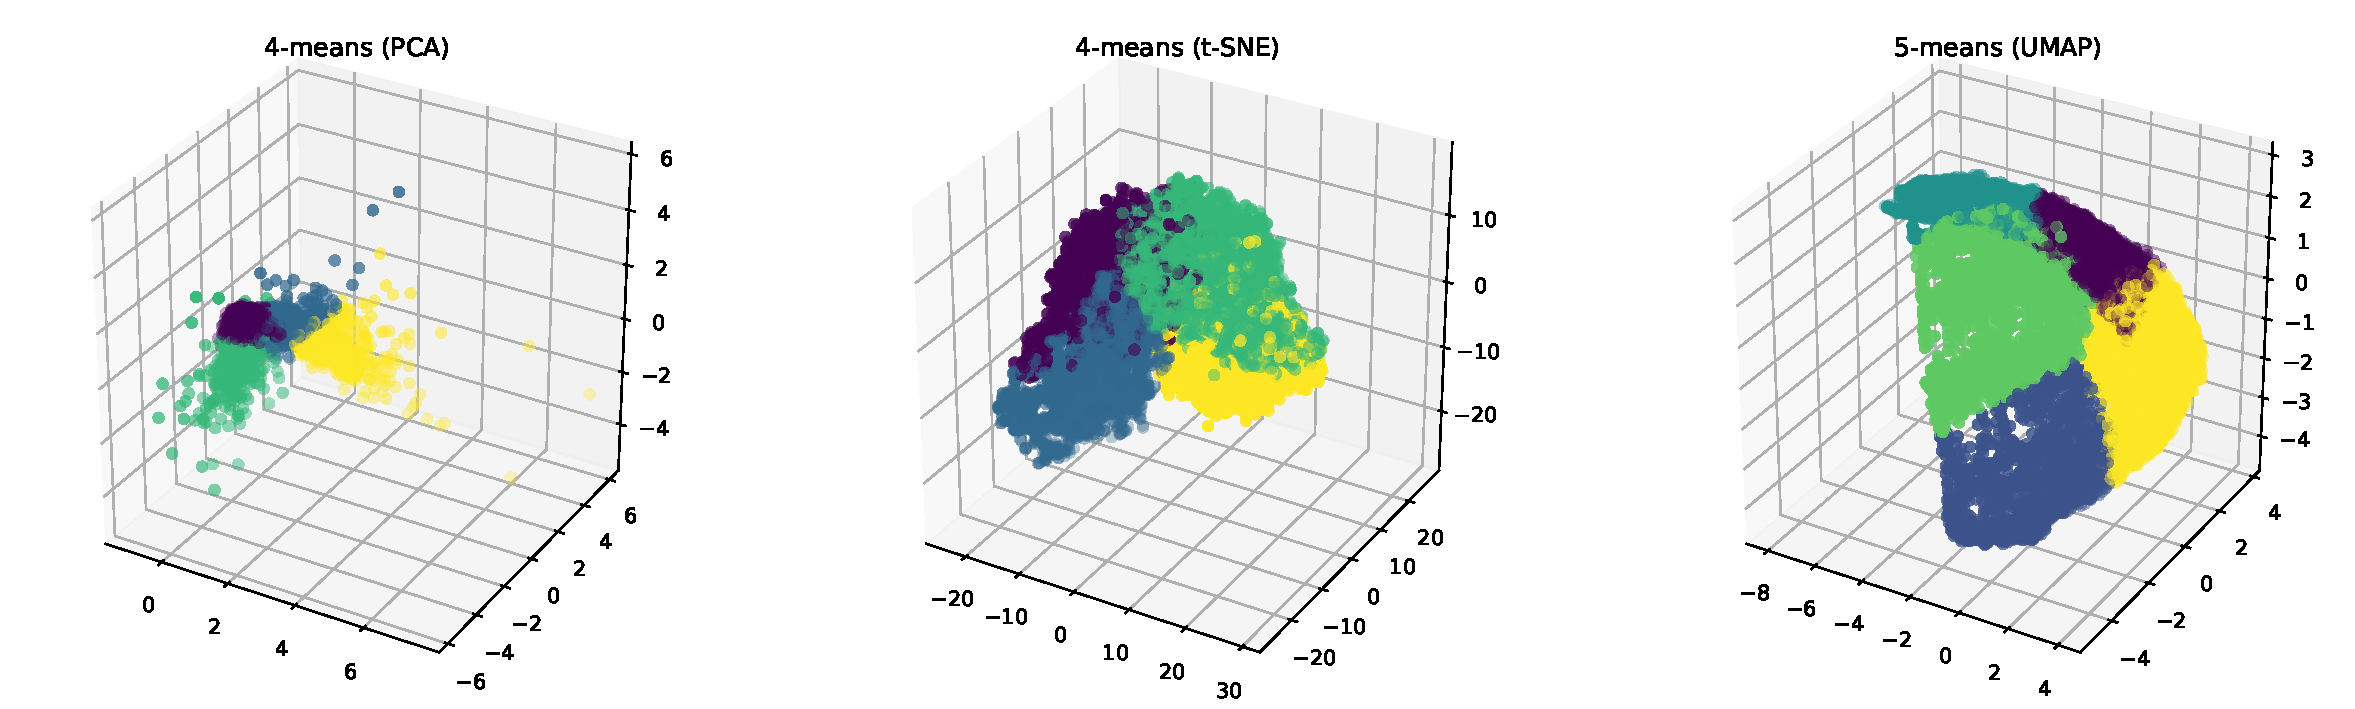
\includegraphics[width=1.0\textwidth]{images/appendix/App8.pdf}\\
	\caption{Resulting $k$-means clustering.}
	\label{fig:App8}
\end{figure}

\section{HDBSCAN}
The sets from~\autoref{fig:App5} were clustered by HDBSCAN as well.~\autoref{fig:App11} suggests the best hyperparameters: PCA - min\_cluster\_size = 20, min\_samples = 5, alpha = 0.25;
t-SNE - min\_cluster\_size = 30, min\_samples = 40, alpha = 0.25; UMAP - min\_cluster\_size = 10, min\_samples = 20, alpha = 0.25.~\autoref{fig:App12} shows the coloured by defined HDBSCAN clusters embeddings. The best clustering according to the set of internal clustering metrics is PCA-reduced embeddings split into 2 clusters (left plot on~\autoref{fig:App12}).

\begin{figure}[!ht]
	\centering
	\includegraphics[width=1.0\textwidth]{images/appendix/App11.pdf}\\
	\caption{Evaluation of HDBSCAN clustering with respect to the set of hyperparameters.}
	\label{fig:App11}
\end{figure}
\begin{figure}[!ht]
	\centering
	\includegraphics[width=1.0\textwidth]{images/appendix/App12.pdf}\\
	\caption{Resulting HDBSCAN clustering.}
	\label{fig:App12}
\end{figure}

\section{Interpretation of the results}
Some initial time analysis was done in appendix 1 (~\autoref{fig:App13} and ~\autoref{fig:App14}). The degree distribution of the initial network is on the~\autoref{fig:App17}. It follows Power law distribution: the majority of nodes have low degrees and minority - high degrees.

~\autoref{fig:App18} shows degree distribution and distribution of nodes by time classes within each of 5 $k$-means clusters of the UMAP-redused set of embeddings. Characteristics of the clusters on the~\autoref{fig:App19} by their degree and time classes distribution on the ~\autoref{fig:App18} (top to bottom):
    \begin{enumerate}
        \item 1902 nodes (violet) - mean 62.4 - std 61.6
        \item 1949 nodes (blue) - mean 46 - std 64.7
        \item 2163 nodes (light green) - mean 12.5 - std 8.4
        \item 2284 nodes (yellow) - mean 49 - std 60.7
        \item 3579 nodes (dark green) - mean 4.8 - std 4.5
    \end{enumerate}
The majority of the nodes with low degrees from all possible time classes are accumulated in the most numerous fifth cluster. The fifth dark green cluster penetrates to the third light green cluster, whose average degree is slightly higher and nodes mostly act in the latest periods. It might be assumed that nodes on the periphery of the network do not tend to connect to hubs of high degree directly, but by paths through nodes of steadily increasing degrees. The degree distribution within the first class is right-skewed with heavy right tail, where the most hubs are. This cluster is not adjacent to the fifth, and this fact supports the above hypothesis about network structure.

Another observation is the second blue cluster consists of nodes being active in the earlier periods. It does not connect to the first violet and the third light green clusters, whose nodes were active mostly in recent periods. The second blue and the fourth yellow clusters adjoin and have a long border, which was hard to spot by the structure of the set. Their degree and time classes distributions are quite similar. 

The closer look at the second blue -> fourth yellow -> first violet clusters in exactly this sequence reveal some insights: 
\begin{itemize}
    \item degree distributions are right-skewed and their means move gradually to the right from blue cluster to the violet over the set.
    \item the time classes distributions within these three clusters are characterised as the earliest active nodes -> active nodes in the middle time period -> active nodes in the recent time periods. This is also reflected in the gradual transition from the blue -> yellow -> violet clusters.
\end{itemize}

The assumptions made above were based mostly on the clusters adjacency in the representation space. The transitions between clusters help to understand what kinds of nodes of the network tend to communicate with each other.
\begin{figure}[!ht]
	\centering
	\includegraphics[width=1.0\textwidth]{images/appendix/App17.pdf}\\
	\caption{Degree distribution of the financial network.}
	\label{fig:App17}
\end{figure}
\begin{figure}[!ht]
	\centering
	\includegraphics[width=0.4\textwidth]{images/appendix/App19.pdf}\\
	\caption{$k$-means ($k$=5) clustering on UMAP-reduced set of embeddings.}
	\label{fig:App19}
\end{figure}
\begin{figure}[!ht]
	\centering
	\includegraphics[width=0.9\textwidth]{images/appendix/App18.pdf}\\
	\caption{Degree and time classes distribution of nodes within each of 5 $k$-means clusters of the UMAP-redused set of embeddings.From the first to the fifth cluster top to bottom.}
	\label{fig:App18}
\end{figure}

